\documentclass[10pt,letterpaper]{article}

\usepackage{hyperref, breakurl}
\usepackage{erinmod_cogsci}
\usepackage{pslatex}
\usepackage{apacite}
\usepackage{graphicx}
\usepackage{caption}
\usepackage{subcaption}
\usepackage{color}
\usepackage{amsfonts}
\usepackage{amsmath}

\newcommand{\w}[1]{\emph{#1}}
\newcommand{\todo}[1]{{\color{red}#1}}

\title{Extremely costly intensifiers are stronger than quite costly ones: Appendix}
 
\author{{\large \bf Erin Bennett} (erindb@stanford.edu), {\large \bf Noah D.~Goodman} (ngoodman@stanford.edu)\\
  Department of Psychology, Stanford University.}
  
\begin{document}

\maketitle
 
\section{Model} \label{app:model}

 \citeA{lassiter}'s model belongs to the family of Rational Speech Act (RSA) models in which speaker and listener communicate by recursively reasoning about each other's goals and inferences. These models have been shown to account for many phenomena in pragmatics
\cite{frank, goodman}. The adjective model accounts for uncertainty about the adjectival threshold by including a lifted semantic variable, which the pragmatic listener infers at the same time that she infers the speaker's intended meaning. 
We assume every adjective phrase has its own such variable $\theta_i$\footnote{Other versions of this model could easily be imagined in which the threshold for an adjective phrase is determined by the basic threshold for the adjective and some transformation on that threshold (e.g. multiplication, addition, etc.) caused by the intensifier. If the transformation is mostly regular, with a single parameter needing to be inferred for each intensifier, and if the values of these parameters are inferred for each adjective phrase, then such a model would be functionally equivalent to the one we describe here.}, together notated $\vec{\theta}$, but to otherwise mean the same thing, so that, for example, \w{expensive}, \w{very expensive} and \w{phenomenally expensive} all denote: $\lambda x . \text{price}(x) > \theta_i$. %unpack?

Given an utterance $u_i$ (e.g. an \w{expensive laptop} or a \w{very expensive laptop}) and a set of thresholds, a literal listener $L_0$ will use Bayesian inference to update his prior beliefs $P(d)$ about the degree $d$ (e.g. the laptop's price) given that the degree is greater than the threshold for that utterance.

$$P_{L_0}(d|u_i, \theta_i) \propto P(d) \cdot \delta_{d > \theta_i}$$

A speaker with the goal of communicating some actual degree $d$ assigns a utility $\mathbb{U}(u_i|d)$ to each utterance such that he prefers utterances which will inform the literal listener, but avoids utterance cost, $C(u_i)$:

$$\mathbb{U}(u_i | d, \vec{\theta}) =  \ln\left(P_{L_0}(d | u_i, \theta_i) \right) - C(u_i) $$

Given a set of alternative utterances (e.g. the speaker might be choosing between saying \w{very expensive} as opposed to \w{expensive} or \w{extremely expensive}, or saying nothing at all), the speaker $S_1$ will choose utterances according to a softmax decision rule \cite{sutton} with optimality parameter $\lambda$, so that:

$$ P_{S_1}(u_i | d, \vec{\theta}) \propto e^{\lambda \mathbb{U}(u_i | d, \vec{\theta})} $$

A pragmatic listener $L_1$ uses the prior probability, $P(d)$, of different degrees, along with knowledge of the cost of each utterance, in order to guess both the thresholds for each utterance and which degree the speaker intended to communicate\footnote{We assume a uniform prior on thresholds $\theta_i$.}:

$$ P_{L_1}(d, \vec{\theta} | u_i) \propto P(d) \cdot P_{S_1}(u_i | d, \vec{\theta}) $$

As an initial exploration, we simulated such a model with three alternative adjective phrases (i.e.~three intensifiers) with costs of $1$, $5$, and $10$. We also included a null utterance, with trivial meaning (always true) and cost of $0$. The prior distribution of degrees along this adjective's scale (which we will discuss as ``prices'' for concreteness and consistency with our Experiment 1) was a gaussian peaked at $0$.
We used an optimality parameter of $\lambda=5$ in our simulation. 

Though the literal semantics are identical (except that they have different threshold parameters), the different phrases received different interpretations: the more costly intensifiers corresponded to less probable, more extreme prices (Figure ~\ref{model}). This can be seen as an M-implicature: more costly intensifiers are assigned strong, less probable, meanings. 
The model therefore predicts an association between intensifier meaning and utterance cost.

\begin{figure}[ht]
\begin{center}
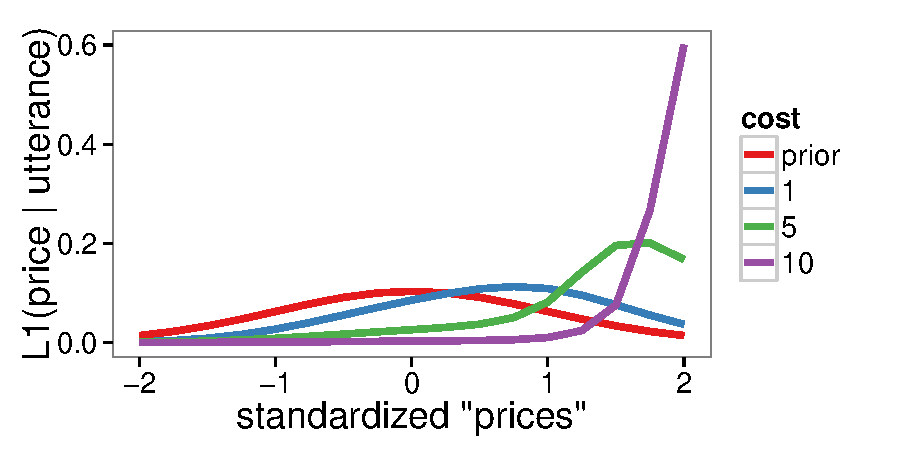
\includegraphics[width=0.4\textwidth]{model_results.pdf}
\end{center}
\caption{Modeling intensifiers as M-implicature: more costly intensifiers correspond to more extreme meanings.} 
\label{model}
\end{figure}

The quantitative form predicted by the model of the relationship between cost and meaning is a approximately linear (Figure \ref{model-heights}).\footnote{This second simulation was identical as the first, except run on a more discretized scale for 6 different utterance costs (or ``intensifiers'').}.

\begin{figure}[ht]
\begin{center}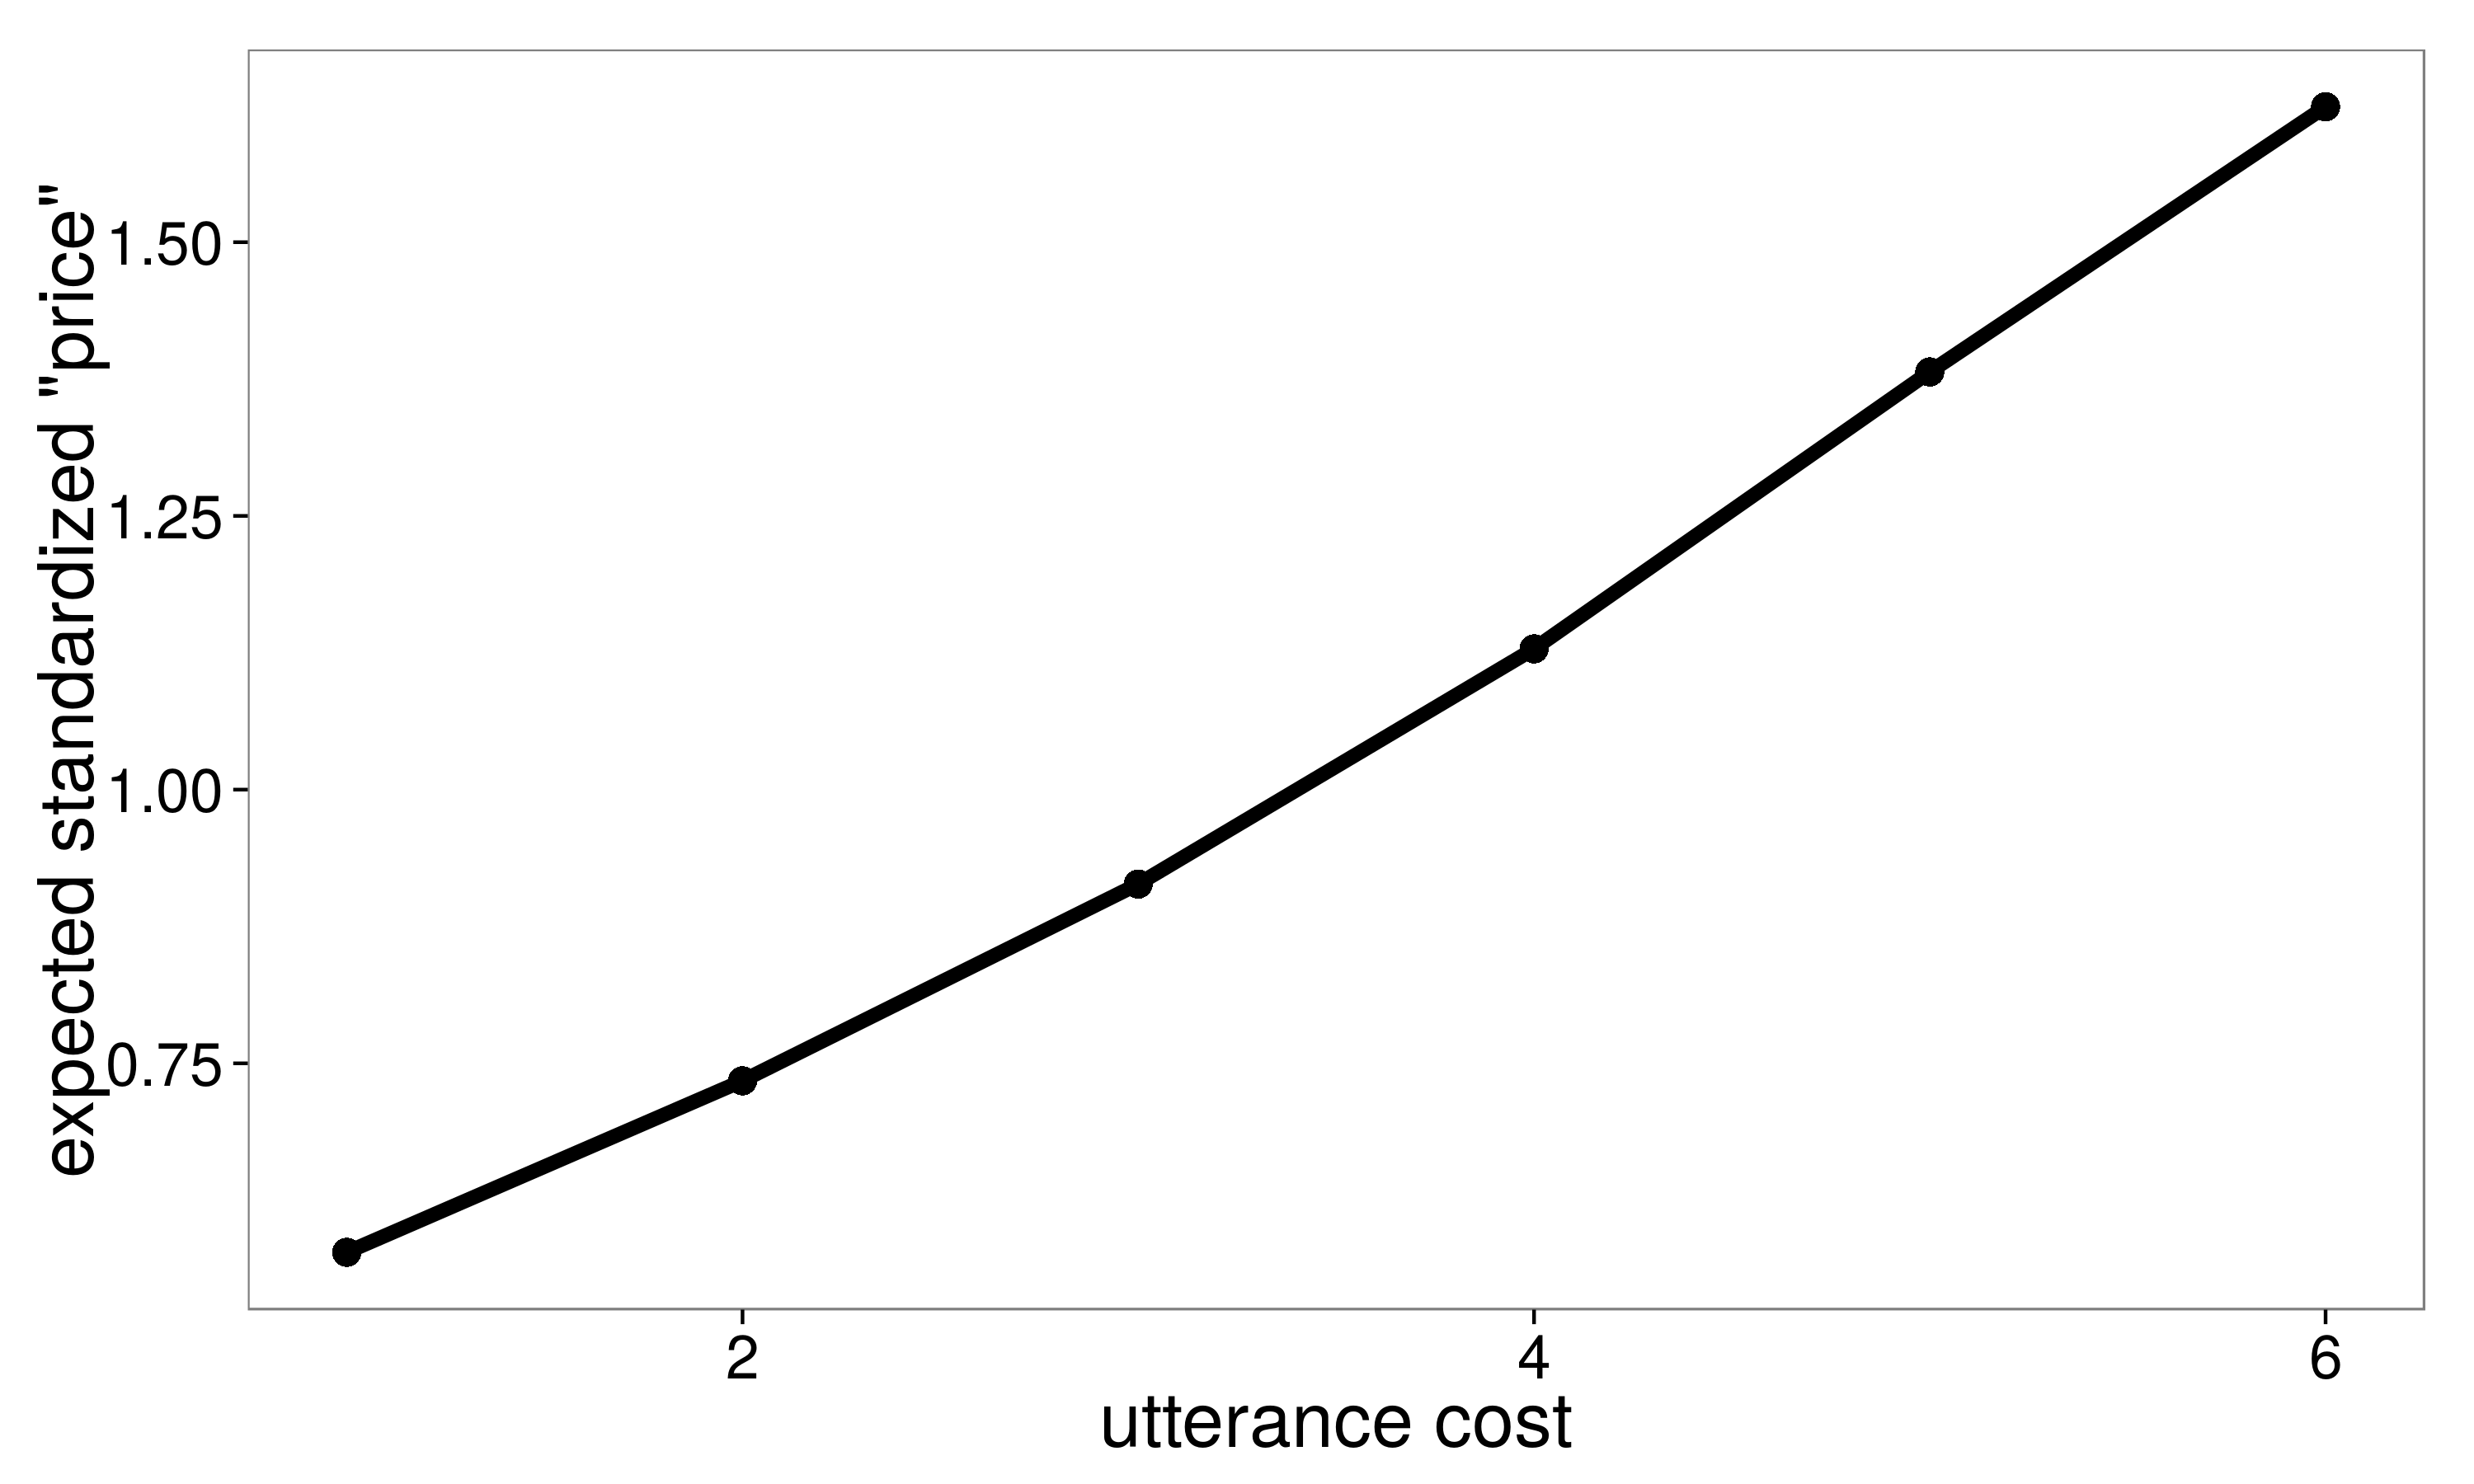
\includegraphics[width=0.4\textwidth]{height-by-cost.png}
\end{center}
\caption{Model prediction of expected price as cost of intensifier increases, based on intensifiers evenly spaced in cost. The relationship is approximately linear.} 
\label{model-heights}
\end{figure}


\bibliographystyle{apacite}

\setlength{\bibleftmargin}{.125in}
\setlength{\bibindent}{-\bibleftmargin}

\bibliography{intensifiers}
 
\end{document}
